\subsection{Sprzęt wizyjny}
Jako bazę do wyznaczania ścieżki robota w~terenie zdecydowano się użyć kamery
\textit{Raspberry Pi Camera V2}, która oferuje obraz wideo w~rozdzielczości
\textit{full HD} oraz zdjęcia w~rozdzielczości do \textit{4K}.
Kamera jest wyposażona we wbudowany obiektyw szerokokątny, co jest korzystne
w~zastosowaniach robotyki.

\subsection{Wyznaczanie przestrzeni ruchów robota}
Kamerę przygotowano do wykorzystania w~celu wykonywania zdjęcia labiryntu,
w~którym poruszać może się robot.
Obraz z~kamery należy przetworzyć aby uzyskać mapę przestrzeni, po której może
poruszać się robot.
Biała przestrzeń na mapie powinna oznaczać miejsca, w których może znaleźć się 
środek robota, czarne pola to miejsca zabronione (przeszkody oraz ich
margines).
Budowę mapy wykonano w~następujących krokach:
\begin{itemize}
	\item binaryzacja zdjęcia z kamery,
	\item wykrycie położenia robota oraz jego promienia na podstawie markerów,
	\item usunięcie obrysu robota z~przestrzeni zabronionej, 
	\item naniesienie marginesu przeszkód.
\end{itemize}

Ze względu na zdalny charakter pracy w~semestrze letnim 2020 przygotowano
prototypowy model labiryntu.
Podstawą przetwarzania obrazu labiryntu jest binaryzacja metodą
\textit{isodata}.
Oparcie wizji na algorytmie binaryzacji wymaga odpowiedniego kontrastu zdjęcia
oraz dobrego oświetlenia labiryntu.
\textit{Isodata} jest adaptacyjną metodą binaryzacji zdjęć, która gwarantuje,
że wartość progowania jest średnią ze średnich wartości ekspozycji podzielonych
fragmentów zdjęcia.
Taki algorytm binaryzacji odpowiada algorytmowi klasteryzacji
\textit{k-średnich}, gdzie \textit{k} wynosi dwa.
Przykładowy labirynt po binaryzacji przedstawiono na rysunku
\ref{fig:maze_bin}.
\begin{figure}
\centering
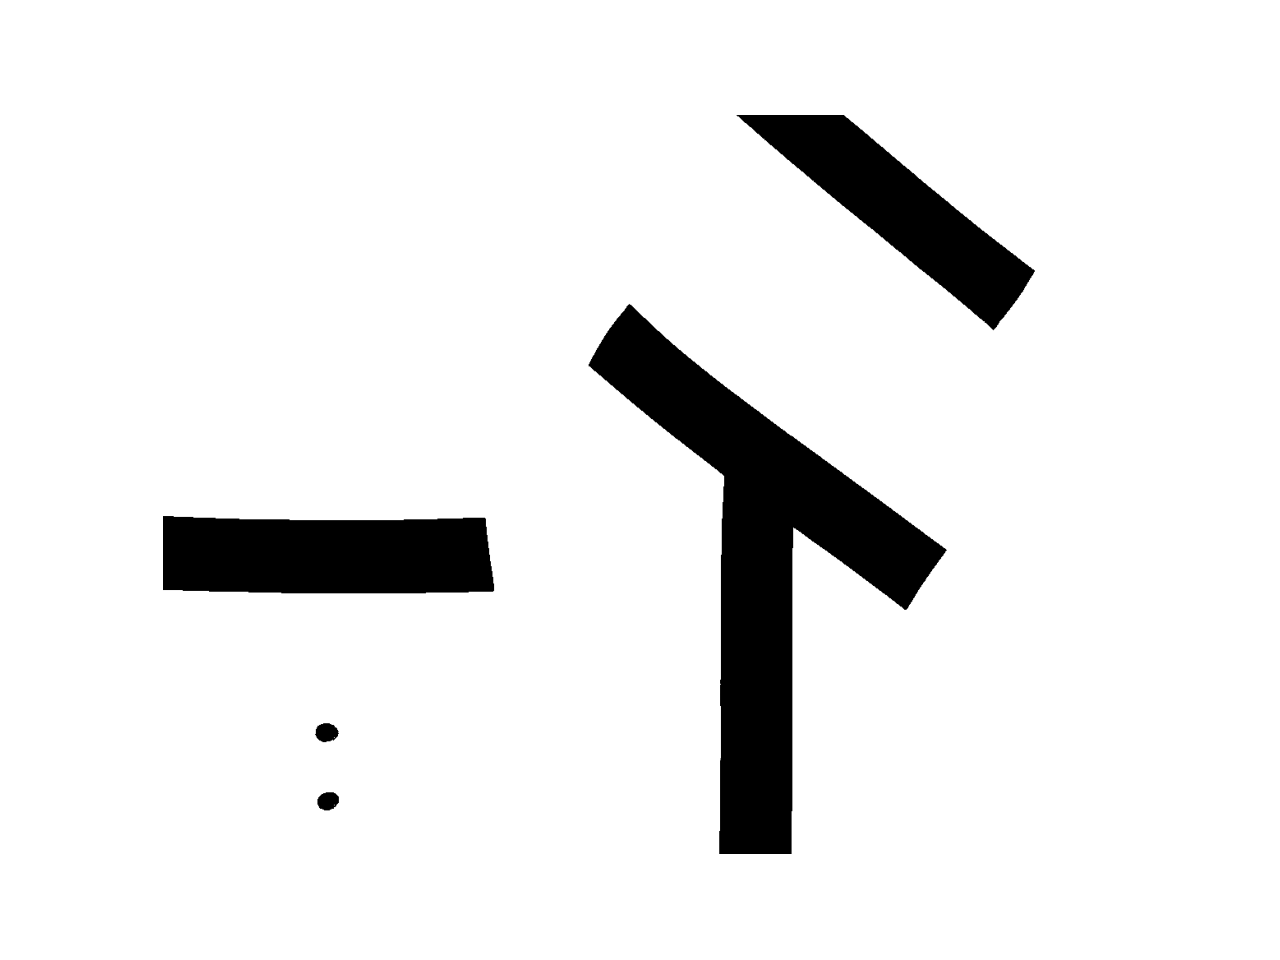
\includegraphics[width=0.5\textwidth]{maze_bin.png}
\caption{Przykładowy labirynt poddany binaryzacji}
\label{fig:maze_bin}
\end{figure}

W~następnym kroku algorytm wizyjny przeprowadza wykrycie pozycji i~rozmiaru
robota na podstawie dwóch czerwonych markerów umieszczonych na jego obwodzie.
Punkty o charakterystycznym kolorze najlepiej wykrywać w~przestrzeni barw HSV
(barwa, nasycenie, jasność ang. \textit{hue, saturation, value}).
W~omawianej przestrzeni kolory są reprezentowane przez wartość kąta; od zera do
kąta pełnego, przy czym wartości reprezentuje często się jako ułamek dziesiętny
z~maksymalnej wartości.
Kolor czerwony jest w~takim systemie opisywany przez kąty zbliżone do zera.
Markery zdecydowano się kwalifikować w~przedziale odcieni czerwonego od 0,9 do
1~oraz 0~do 0,1.
Wartości nasycenia oraz jasności markerów są akceptowane dla wartości większych
od 0,3.
Po progowaniu pozycji markerów dokończono proces ich segmentacji przez
etykietowanie oraz obliczenie parametrów obszaru zajmowanego przez markery.
Wyznaczono ich centroidy; punkt między centroidami markerów to środek robota.
Po wyznaczeniu pozycji robota można usunąć jego kształt z~mapy przez odjęcie
maski jego obrysu z obrazu.
Wyniki omówionych operacji przedstawiono na rysunkach \ref{fig:maze_markers}
oraz \ref{fig:maze_rm_markers}.
\begin{figure}
\centering
\hfill
\begin{subfigure}[b]{0.45\textwidth}
	\centering
	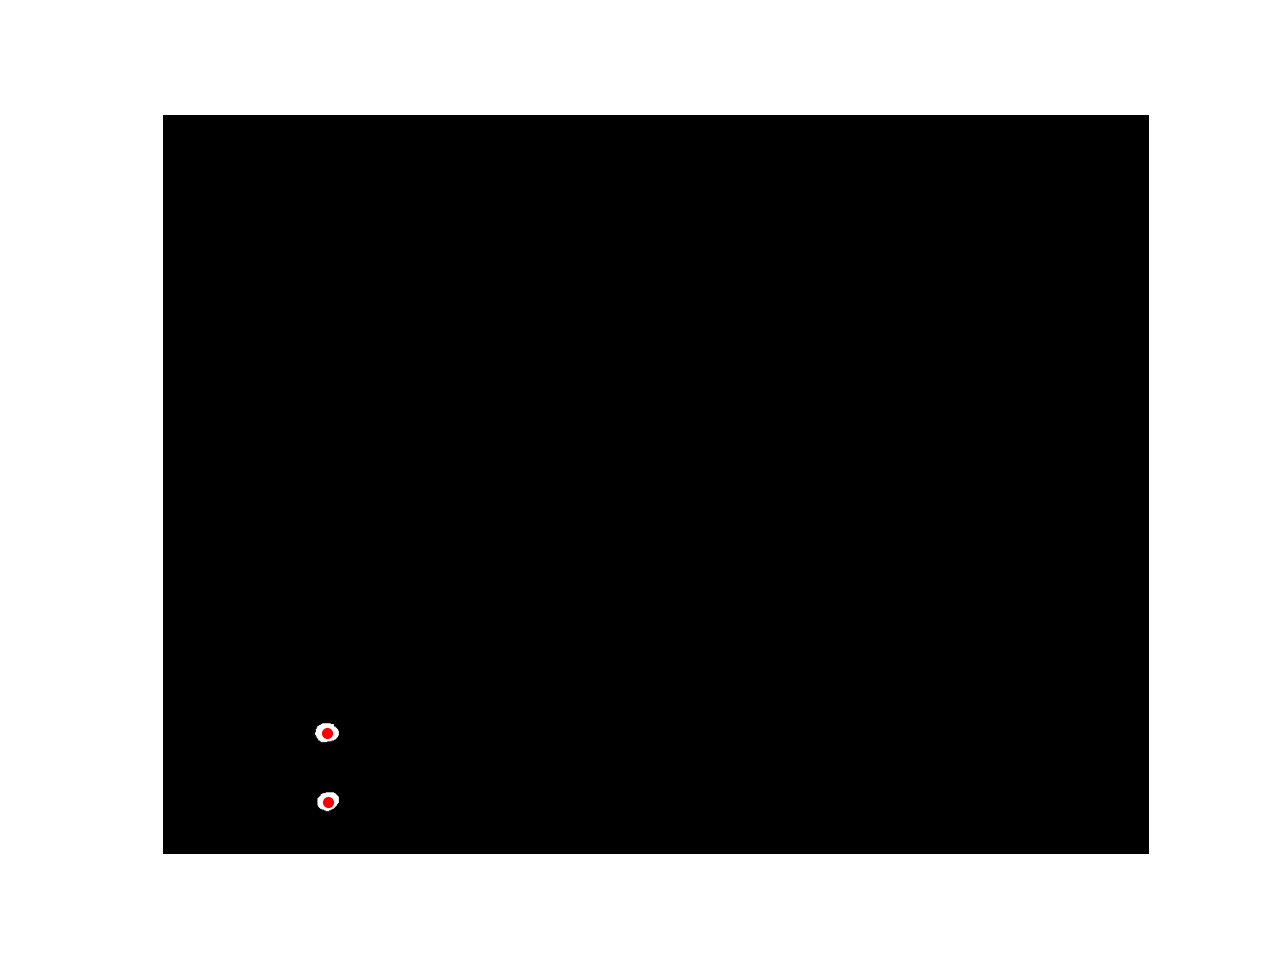
\includegraphics[width=\textwidth]{maze_markers.png}
	\caption{Wykryte markery i~ich centroidy}
	\label{fig:maze_markers}
\end{subfigure}
\hfill
\begin{subfigure}[b]{0.45\textwidth}
	\centering
	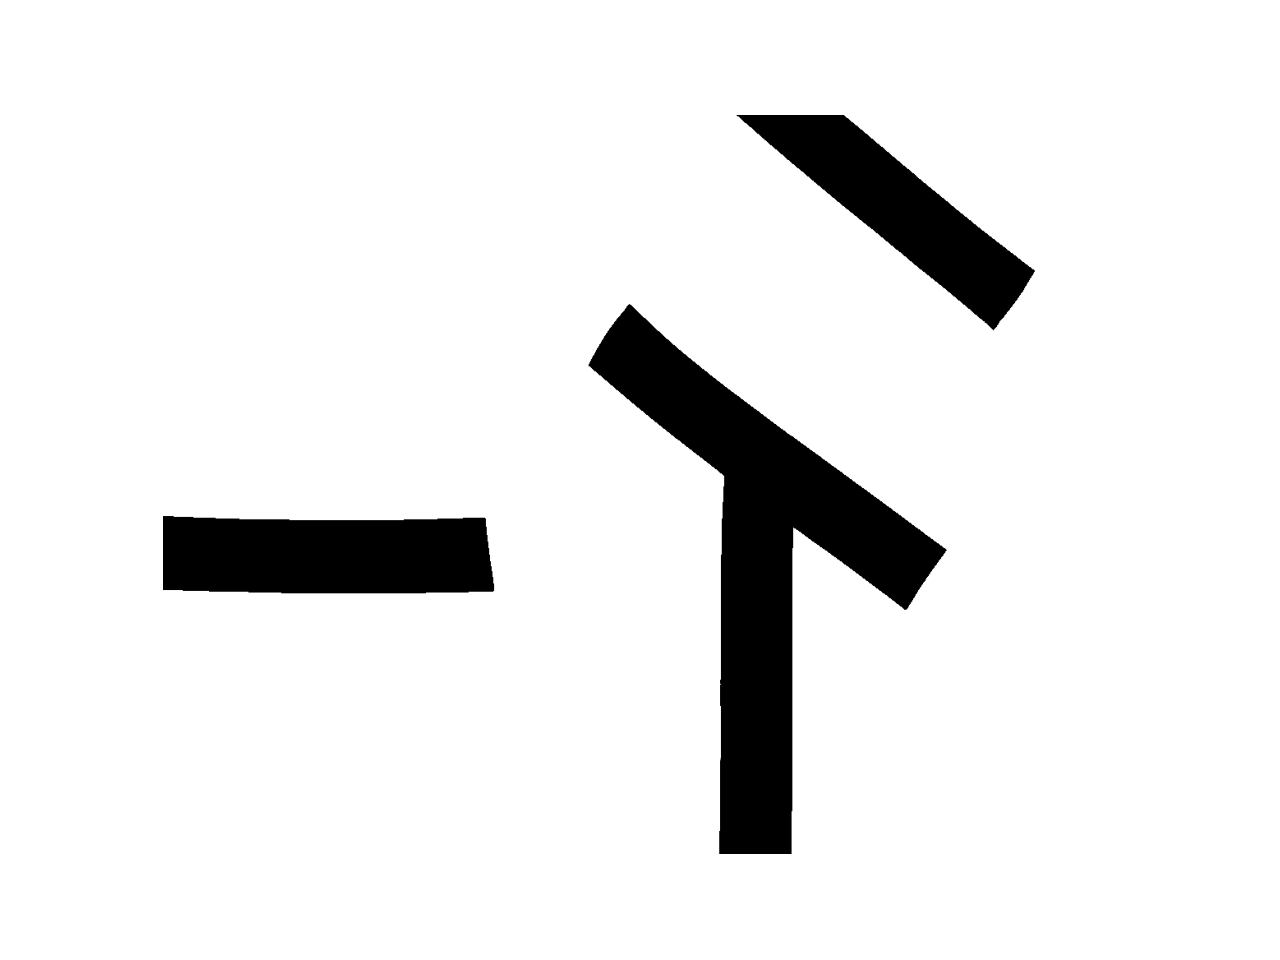
\includegraphics[width=\textwidth]{maze_rm_markers.png}	
	\caption{Labirynt po usunięciu markerów}
	\label{fig:maze_rm_markers}
\end{subfigure}
\hfill
\caption{Wykrywanie oraz usuwanie markerów z~mapy labiryntu}
\end{figure}

Ostatni etap przygotowania mapy polega na dodaniu do ścian labiryntu marginesu,
który zapewni, że krawędź robota nie zetknie się z przeszkodami.
W~tym celu dokonano procesu erozji binarnej przestrzeni dozwolonej ruchu
robota.
Margines ścian wyznaczono na podstawie średnicy robota wyznaczonej przy
segmentacji markerów.
Erozji dokonano używając jądra w~kształcie okręgu o~promieniu równym ponad
połowie promienia robota.
Ostatecznie powstaje mapa binarna, na której kolor biały oznacza przestrzeń
w~której może znaleźć się środek robota, przedstawiono ją na rysunku
\ref{fig:maze_walls}
\begin{figure}
\centering
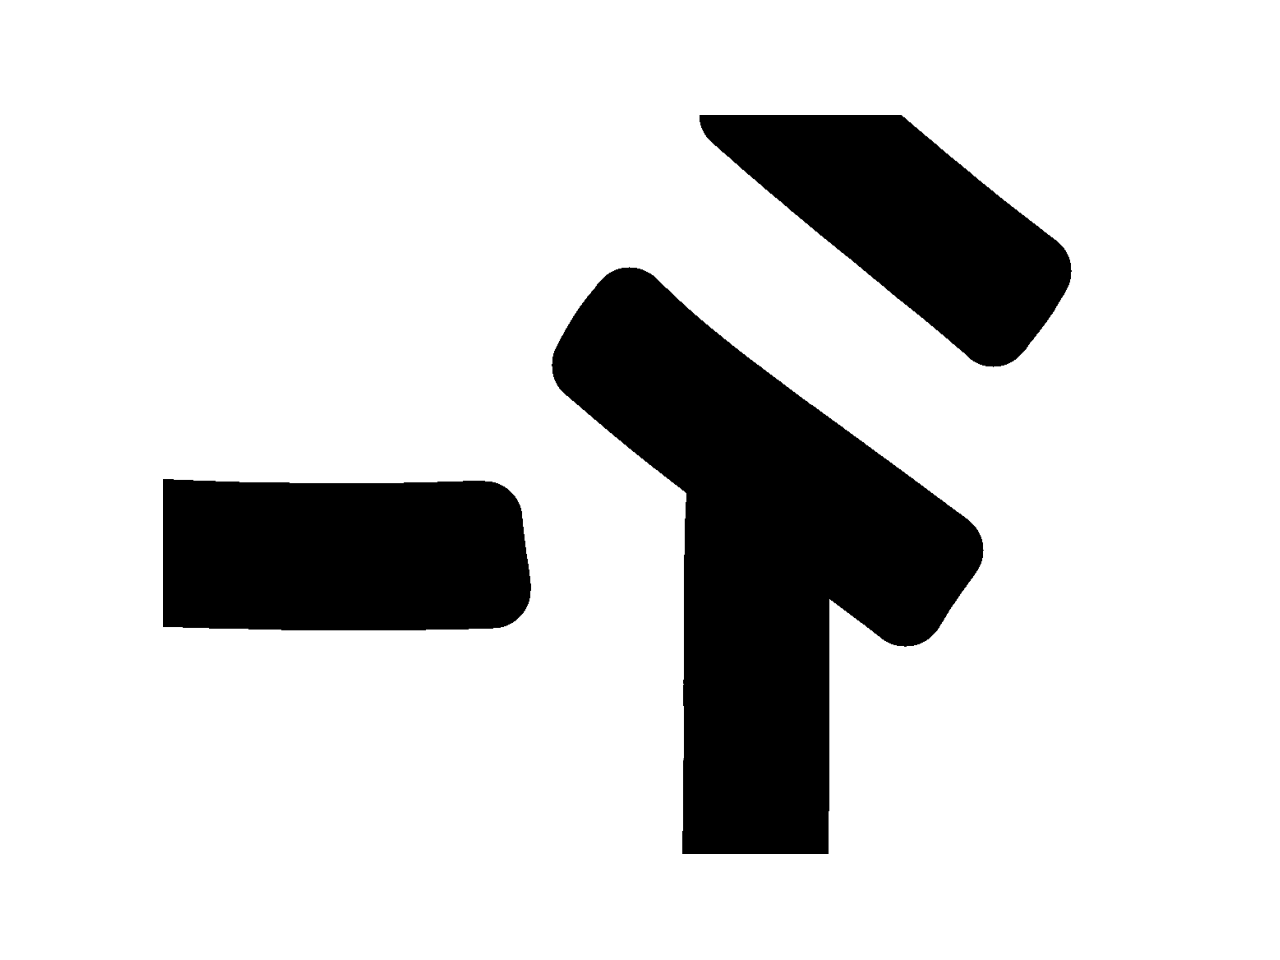
\includegraphics[width=0.5\textwidth]{maze_walls}
\caption{Przykładowy labirynt z~naniesionym marginesem ścian}
\label{fig:maze_walls}
\end{figure}

Do wykonania wymienionych operacji użyto funkcji z~biblioteki
\textit{scikit-image} dla języka Python.